40. $\cfrac{1}{x-2}+\cfrac{1}{x-1}\geqslant\cfrac{1}{x}\Leftrightarrow \cfrac{x(x-1)+x(x-2)-(x-1)(x-2)}{x(x-1)(x-2)}\geqslant0\Leftrightarrow$\\$
\cfrac{x^2-x+x^2-2x-x^2+2x+x-2}{x(x-1)(x-2)}\geqslant0\Leftrightarrow\cfrac{(x-\sqrt{2})(x+\sqrt{2})}{x(x-1)(x-2)}\geqslant0.$\\ Применив метод интервалов, найдём ответ:
\begin{figure}[ht!]
\center{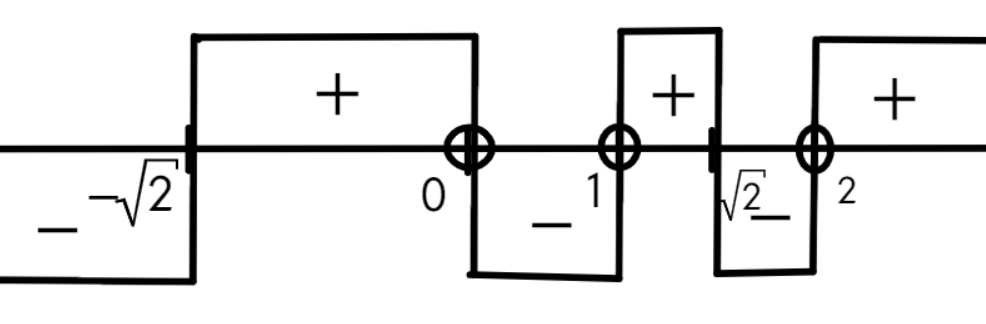
\includegraphics[scale=0.35]{int40.png}}
\end{figure}
$x\in[-\sqrt{2};0)\cup(1;\sqrt{2}]\cup(2;+\infty).$\\
